\documentclass[14pt,a4paper,report]{report}
\usepackage[a4paper, mag=1000, left=2.5cm, right=1cm, top=2cm, bottom=2cm, headsep=0.7cm, footskip=1cm]{geometry}
\usepackage[utf8]{inputenc}
\usepackage[english,russian]{babel}
\usepackage{indentfirst}
\usepackage[dvipsnames]{xcolor}
\usepackage[colorlinks]{hyperref}
\usepackage{listings} 
\usepackage{fancyhdr}
\usepackage{caption}
\usepackage{amsmath}
\usepackage{graphicx}
\usepackage{amsmath}
\usepackage{booktabs}
\usepackage{array}
\newcolumntype{P}[1]{>{\centering\arraybackslash}p{#1}}
\hypersetup{
	colorlinks = true,
	linkcolor  = black
}

\usepackage{titlesec}
\titleformat{\chapter}
{\Large\bfseries} % format
{}                % label
{0pt}             % sep
{\huge}           % before-code


\DeclareCaptionFont{white}{\color{white}} 

% Listing description
\usepackage{listings} 
\DeclareCaptionFormat{listing}{\colorbox{gray}{\parbox{\textwidth}{#1#2#3}}}


\captionsetup[lstlisting]{format=listing,labelfont=white,textfont=white}
\lstset{ 
	% Listing settings
	inputencoding = utf8,			
	extendedchars = \true, 
	keepspaces = true, 			  	 % Поддержка кириллицы и пробелов в комментариях
	language = C,            	 	 % Язык программирования (для подсветки)
	basicstyle = \small\sffamily, 	 % Размер и начертание шрифта для подсветки кода
	                keywordstyle=\color{blue}\ttfamily,
                stringstyle=\color{red}\ttfamily,
                commentstyle=\color{green}\ttfamily,
                morecomment=[l][\color{magenta}]{\#},
	numbers = left,               	 % Где поставить нумерацию строк (слева\справа)
	numberstyle = \tiny,          	 % Размер шрифта для номеров строк
	stepnumber = 1,               	 % Размер шага между двумя номерами строк
	numbersep = 5pt,              	 % Как далеко отстоят номера строк от подсвечиваемого кода
	backgroundcolor = \color{white}, % Цвет фона подсветки - используем \usepackage{color}
	showspaces = false,           	 % Показывать или нет пробелы специальными отступами
	showstringspaces = false,    	 % Показывать или нет пробелы в строках
	showtabs = false,           	 % Показывать или нет табуляцию в строках
	frame = single,              	 % Рисовать рамку вокруг кода
	tabsize = 2,                  	 % Размер табуляции по умолчанию равен 2 пробелам
	captionpos = t,             	 % Позиция заголовка вверху [t] или внизу [b] 
	breaklines = true,           	 % Автоматически переносить строки (да\нет)
	breakatwhitespace = false,   	 % Переносить строки только если есть пробел
	escapeinside = {\%*}{*)}      	 % Если нужно добавить комментарии в коде
}

\begin{document}

\def\contentsname{Содержание}

% Titlepage
\begin{titlepage}
	\begin{center}
		\textsc{Санкт-Петербургский Политехнический 
			Университет Петра Великого\\[5mm]
			Кафедра компьютерных систем и программных технологий}
		
		\vfill
		
		\textbf{Отчёт по лабораторной работе №2\\[3mm]
		на тему: «Методы сглаживания изображений»\\[3mm]
			Курс: «Разработка графических приложений»\\[41mm]
		}
	\end{center}
	
	\hfill
	\begin{minipage}{.4\textwidth}
		Выполнил студент:\\[2mm] 
		Ерниязов Т.Е.\\
		Группа: 13541/2\\[5mm]
		
		Проверил:\\[2mm] 
		Абрамов Н.А.
	\end{minipage}
	\vfill
	\begin{center}
		Санкт-Петербург\\ \the\year\ г.
	\end{center}
\end{titlepage}

% Contents
\tableofcontents
\clearpage

\chapter{Лабораторная работа №2}

\section{Цель работы}

Ознакомится с методами сглаживания, на таких подходах, как: Gaussian Blur; Bilateral Filter; Non – local means.

\section{Программа работы}

\begin{enumerate}
\item Реализовать следующие методы сглаживания изображений на языке с++:
\begin{itemize}
\item Gaussian Blur
\item Bilateral Filter
\item Non – local means.
\end{itemize}
\item Сравнить результаты со стандартными функциями библиотеки opencv.
\item Сравнить работу.
\item Результаты привести в отчет.
\end{enumerate}


\clearpage

\section{Ход работы}

\subsection{Фильтр Гаусса}
Фильтр Гаусса —фильтр, чьей импульсной переходной функцией является функция Гаусса. Фильтр Гаусса (Gaussian filter) обычно используется в цифровом виде для обработки двумерных сигналов (изображений) с целью снижения уровня шума. Однако при ресемплинге он дает сильное размытие изображения. 
Гауссова функция (гауссиан, гауссиана, функция Гаусса) — вещественная функция, описываемая следующей формулой:

$$ g(x) = a*exp^{-\dfrac{(x-b)^2}{2c^2}} $$
Это наиболее часто используемый метод размытия. Мы можем использовать этот фильтр для устранения шумов на изображении. Но нам нужно быть очень осторожными в выборе размера ядра и стандартного отклонения распределения Гаусса по X и Y направлению. Они должны быть тщательно подобраны.

GaussianBlur() синтакс:

\begin{lstlisting}
void GaussianBlur(InputArray src, OutputArray dst, Size ksize, double sigmaX, double sigmaY=0, int borderType=BORDER_DEFAULT )
\end{lstlisting}
Параметры:
\begin{itemize}
\item src - входное изображение; изображение может иметь любое количество каналов, которые обрабатываются независимо друг от друга.

\item dst — выходное изображение тогоже размера и типа, что и src.

\item ksize — размер Гауссова ядра. ksize.width и ksize.height могут отличаться, но они оба должны быть положительными и нечетным. 

\item sigmaX — стандартное отклонение Гауссова ядра в направлении X.

\item sigmaY — стандартное отклонение Гауссова ядра в Y направлении; если sigmaY равен нулю, то устанавливается равным sigmaX, если оба сигмы нули, они вычисляются из ksize.width и ksize.height, соответственно; для тогоб чтобы полностью контролировать результат, независимо от возможных будущих модификаций, рекомендуется указать все ksize, sigmaX и sigmaY.

\item borderType — пиксельный метод экстраполяции.
\end{itemize}

Возьмем тестовое изображение:
\begin{figure}[h!]
	\centering
	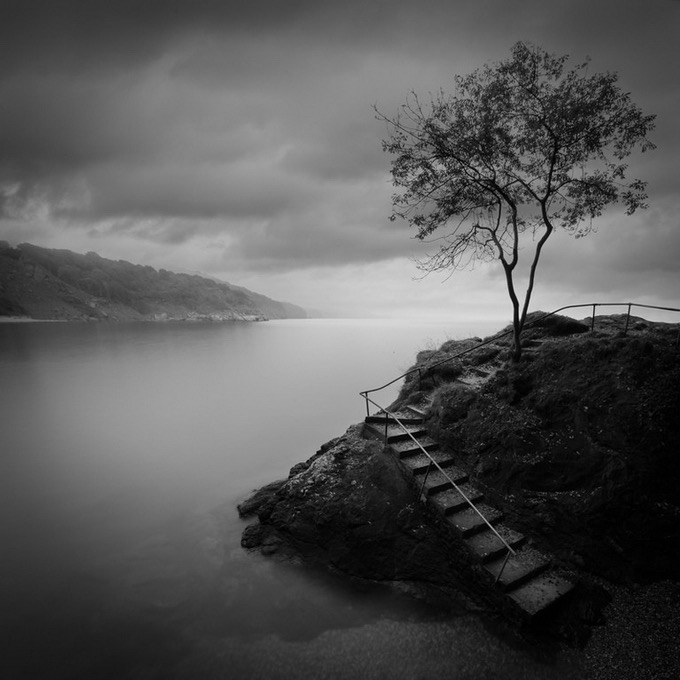
\includegraphics[scale = 0.3]{images/orig.jpg}
	\caption{Тестовое изображение}
\end{figure}



\clearpage

Добавим на него легкий шум:
\begin{figure}[h!]
	\centering
	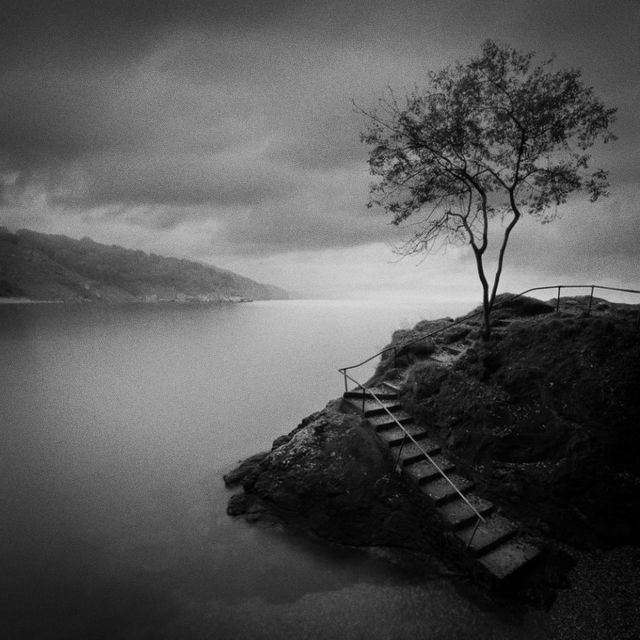
\includegraphics[scale = 0.3]{images/noise.jpg}
	\caption{Изображение с шумом}
\end{figure}

Полный код программы представленн в листинге. Применим фильтр для изображения и сравним с стандартной функцией opencv:
\begin{figure}[h]
\begin{minipage}[h]{0.47\linewidth}
\center{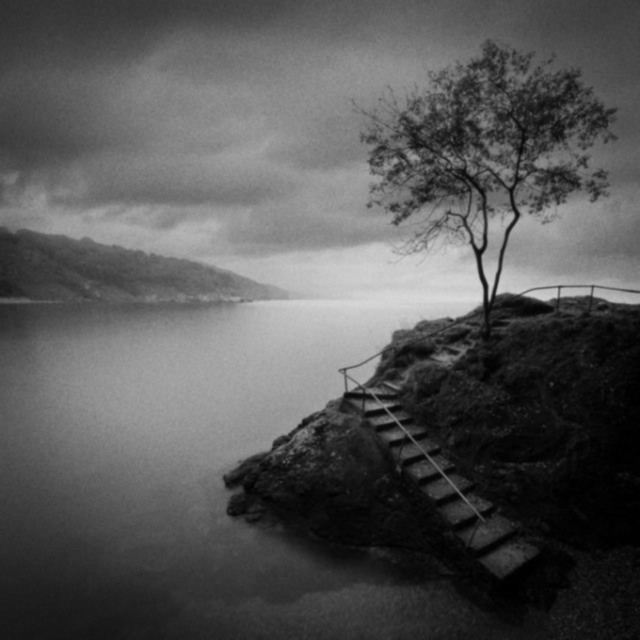
\includegraphics[width=1\linewidth]{images/GB_ocv_sigma_08.png} \\ а) GaussianBlur} 
\end{minipage}
\hfill
\begin{minipage}[h]{0.47\linewidth}
\center{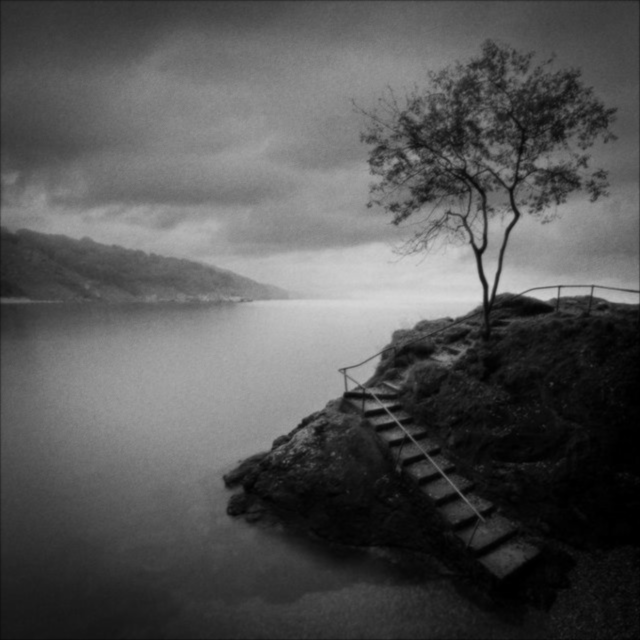
\includegraphics[width=1\linewidth]{images/GB_sigma_08.png} \\ б) GaussFilterOwn}
\end{minipage}
\caption{Изображение после применения фильтра Гаусса (sigma = 0.8)}
\label{ris:image1}
\end{figure}
\clearpage

Для лучшего понимания работы фильтра и для более резкого результата, увеличим значение сигмы:
 
\begin{figure}[h]
\begin{minipage}[h]{0.47\linewidth}
\center{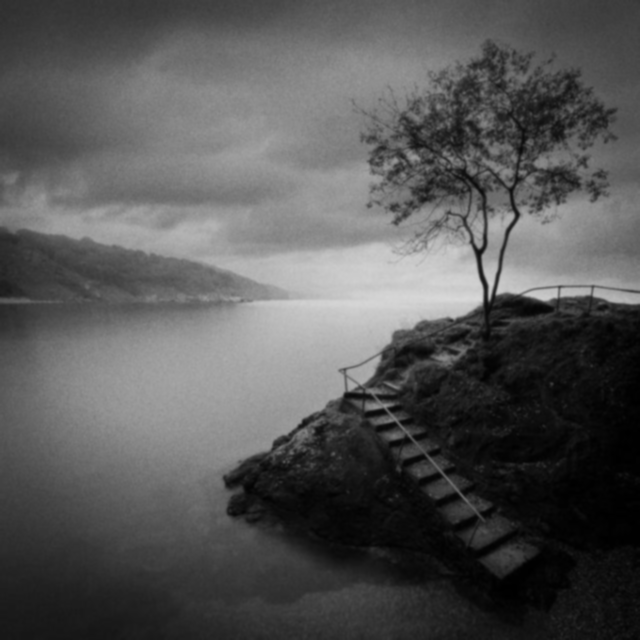
\includegraphics[width=1\linewidth]{images/GB_ocv_sigma_1.png} \\ а) GaussianBlur} 
\end{minipage}
\hfill
\begin{minipage}[h]{0.47\linewidth}
\center{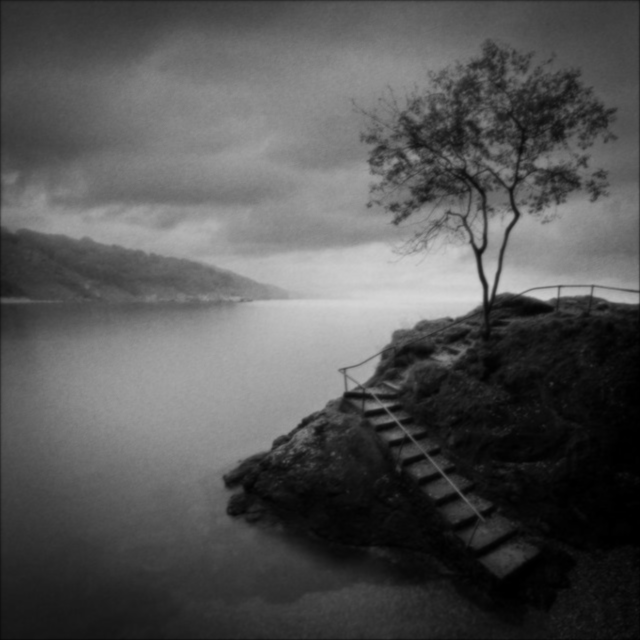
\includegraphics[width=1\linewidth]{images/GB_sigma_1.png} \\ б) GaussFilterOwn}
\end{minipage}
\caption{Изображение после применения фильтра Гаусса (sigma = 1)}
\label{ris:image1}
\end{figure}

На изображениях видно, что фильтр прекрасно справился с удалением шума, без потери четкости и элементов изображений, а результат кастомного фильтра практически не различается с фильтром из библиотеки opencv.




\subsection{Билатеральный фильтр}
Введённый Tomasi и Manduchi билатеральный фильтр, сохраняющий края, нашёл широкое применение во многих задачах по обработке изображений, например, фильтрация шума , редактирование текстуры и тона, оценки оптического потока. Билатеральная фильтрация также часто используется в качестве начального этапа обработки кадров, например, для задачи распознавания объектов, где необходимо отфильтровать несущественные детали и шумы при сохранении резких краев основного изображения. Основным недостатком билатеральных фильтров являются большие вычислительные затраты. Билатеральная фильтрация (двунаправленная фильтрация) - это нелинейный и не итерационный процесс, комбинирующий пространственную (domain) и яркостную (range) фильтрацию. Таким образом, учитывается не только значения интенсивности близлежащих пикселей, но и их расстояние до текущего фильтруемого пикселя. Вклад близлежащих пикселей существенен по отношению к остальным.

bilateralFilter() синтаксис:

\begin{lstlisting}
void bilateralFilter(InputArray src, OutputArray dst, int d, double sigmaColor, double sigmaSpace, int borderType=BORDER_DEFAULT )
\end{lstlisting}

\begin{itemize}

\item src – входное изображение.

\item dst – выходное изображение того же формата, что и src .

\item d – диаметр каждой пиксельной окрестности, которая используется во время фильтрации. Если оно не положительное, оно вычисляется из sigmaSpace .

\item sigmaColor – Фильтр сигма в цветовом пространстве. Большее значение параметра означает, что более дальние цвета в SigmaSpace будут смешаны вместе, что приведет к большим областям с полурастворенным цветом.

\item sigmaSpace – Фильтр сигма в координатном пространстве. Большее значение параметра означает, что дальнейшие пиксели будут влиять друг на друга, пока SigmaColor достаточно близки. Когда d>0, он определяет размер окрестности независимо от sigmaSpace. В противном случае, d пропорционально sigmaSpace.
\end{itemize}

Как подсказывает документация, легким способом подбора значений сигм - установить их одинаковыми. Большое значение сигмы (> 150) обещает удалить все шумы, но это означет потерю четкости и эффект "мультяшности".

Большие фильтры (d> 5) очень медленные, поэтому рекомендуется использовать d = 5 и, возможно, d = 9 для автономных приложений.

Стремление sigma к нулю делает билатеральный фильтр простым сглаживающим фильтром Гаусса.


Посмотрим результаты:


\begin{figure}[h]
\begin{minipage}[h]{0.47\linewidth}
\center{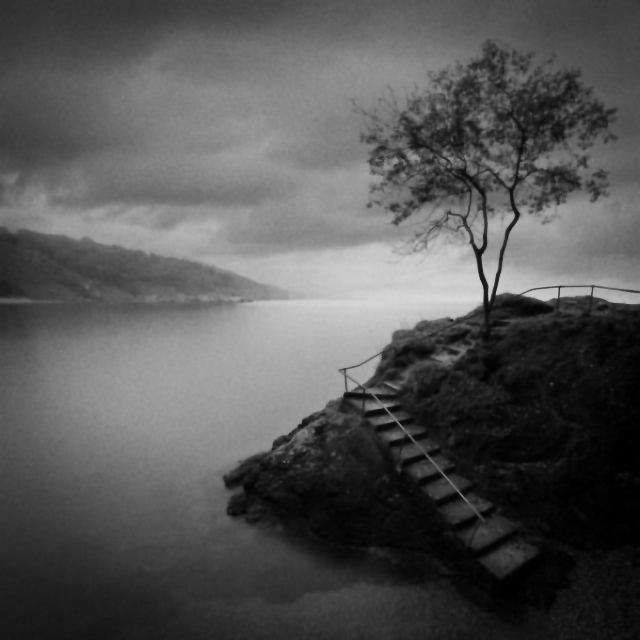
\includegraphics[width=1\linewidth]{images/b_op_5_50_50.png} \\ а) bilateralFilter} 
\end{minipage}
\hfill
\begin{minipage}[h]{0.47\linewidth}
\center{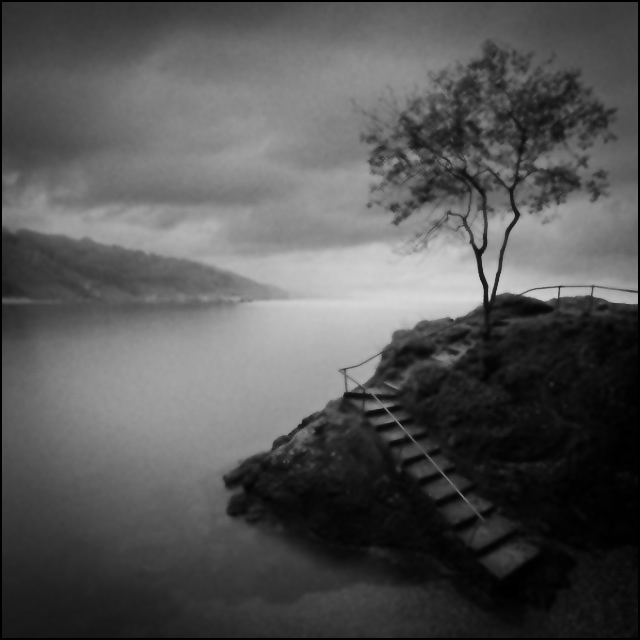
\includegraphics[width=1\linewidth]{images/b_5_50_50.png} \\ б) BilateralFilterOwn}
\end{minipage}
\caption{Изображение после применения билатерального фильтра (d = 5, sigma = 50)}
\label{ris:image1}
\end{figure}

\clearpage
Увеличим значения параметров, для большей презентабельности:

\begin{figure}[h]
\begin{minipage}[h]{0.47\linewidth}
\center{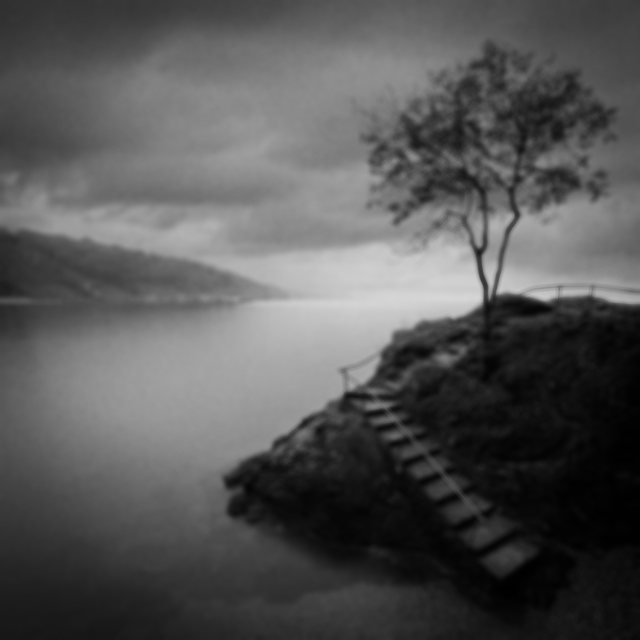
\includegraphics[width=1\linewidth]{images/b_op_9_150_150.png} \\ а) bilateralFilter} 
\end{minipage}
\hfill
\begin{minipage}[h]{0.47\linewidth}
\center{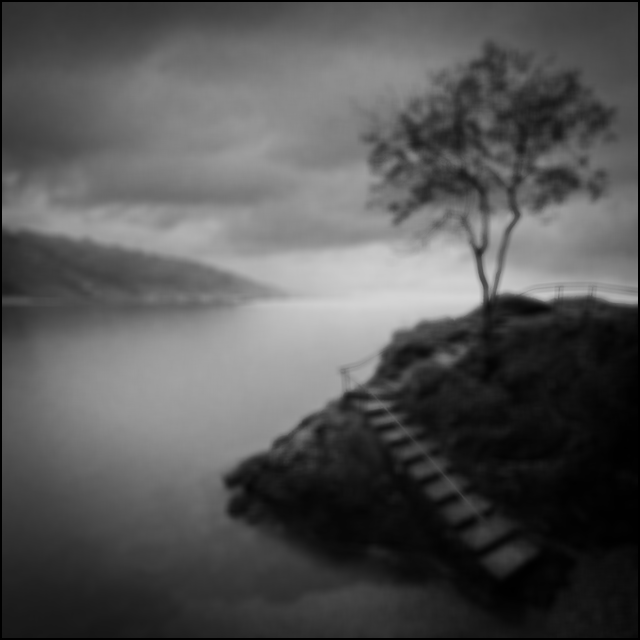
\includegraphics[width=1\linewidth]{images/b_9_150_150.png} \\ б) BilateralFilterOwn}
\end{minipage}
\caption{Изображение после применения билатерального фильтра (d = 9, sigma = 150)}
\label{ris:image1}
\end{figure}

Билетеральный фильтр также не плохо справился с подавлением шума.


\subsection{Фильтр NLMeans}

Это алгоритм обработки изображений для шумоподавления. В отличие от фильтров" local mean", которые принимают среднее значение группы пикселей, окружающих целевой пиксель, для сглаживания изображения, фильтрация нелокальными средствами принимает среднее значение всех пикселей в изображении, взвешенное по тому, насколько похожи эти пиксели на целевой пиксель. Это приводит к гораздо большей ясности постфильтрации и меньшей потере деталей изображения по сравнению с локальными средними алгоритмами. По сравнению с другими известными методами шумоподавления нелокальные средства добавляют "методический шум" (т. е. ошибку в процессе шумоподавления), который больше похож на белый шум, что желательно, поскольку он обычно менее тревожен в шумоизолированном продукте. 
Цель весовой функции-определить, насколько тесно изображение в точке p связано с изображением в точке q. Она может принимать различные формы. 
Весовая функция Гаусса

$$ f(p,q) = exp^{-\dfrac{ |B(q)-B(p) |^2}{h^2}} $$

fastNlMeansDenoising() синтаксис:

\begin{lstlisting}
void fastNlMeansDenoising(InputArray src, OutputArray dst, float h, int templateWindowSize, int searchWindowSize )
\end{lstlisting}
Параметры:
\begin{itemize}
\item src – входное изображение.

\item dst – выходное изображение того же формата, что и src .

\item templateWindowSize - размер в пикселях патча шаблона, который используется для вычисления весов. 

\item searchWindowSize - размер в пикселях окна, который используется для вычисления средневзвешенного значения для данного пикселя.  Линейно влияет на производительность. Чем больше searchWindowsSize, тем больше время удаления шума. 
\item h - параметр, регулирующий силу фильтра. Большое значение h идеально удаляет шум, но также удаляет детали изображения, меньшее значение h сохраняет детали, но также сохраняет шум
\end{itemize}

\clearpage
Также есть функция fastNlMeansDenoisingColored(), которая удаляет шум на цветных изображениях.

Посмотрим результаты:

\begin{figure}[h]
\begin{minipage}[h]{0.47\linewidth}
\center{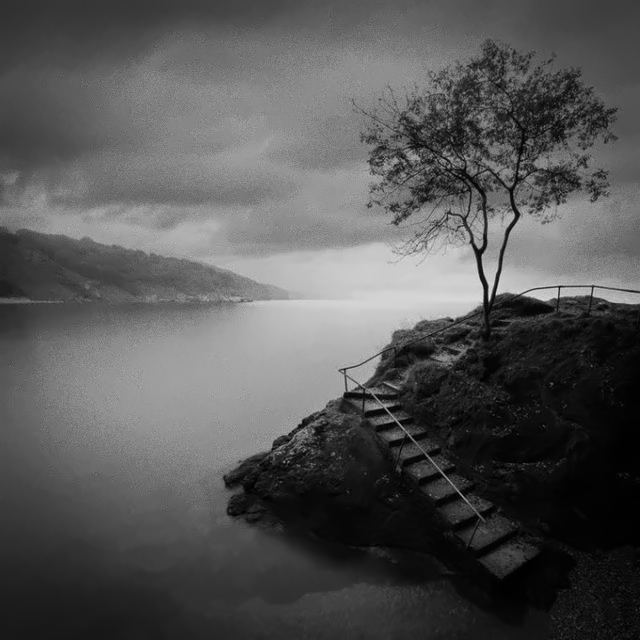
\includegraphics[width=1\linewidth]{images/NLM_op_3_7_21.png} \\ а) fastNlMeansDenoising} 
\end{minipage}
\hfill
\begin{minipage}[h]{0.47\linewidth}
\center{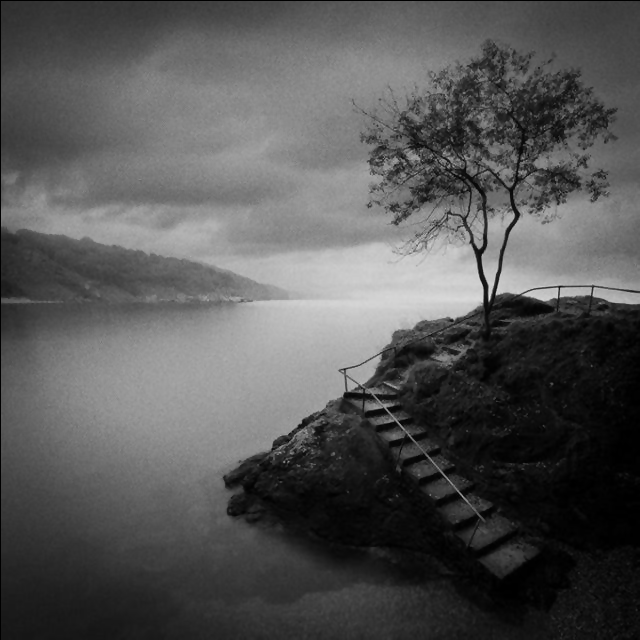
\includegraphics[width=1\linewidth]{images/NLM_3_15.png} \\ б) NLMeansFilterOwn}
\end{minipage}
\caption{Изображение после применения фильтра NLMeans (d = 3, sigma = 15)}
\label{ris:image1}
\end{figure}

Увеличим значения параметров:

\begin{figure}[h]
\begin{minipage}[h]{0.47\linewidth}
\center{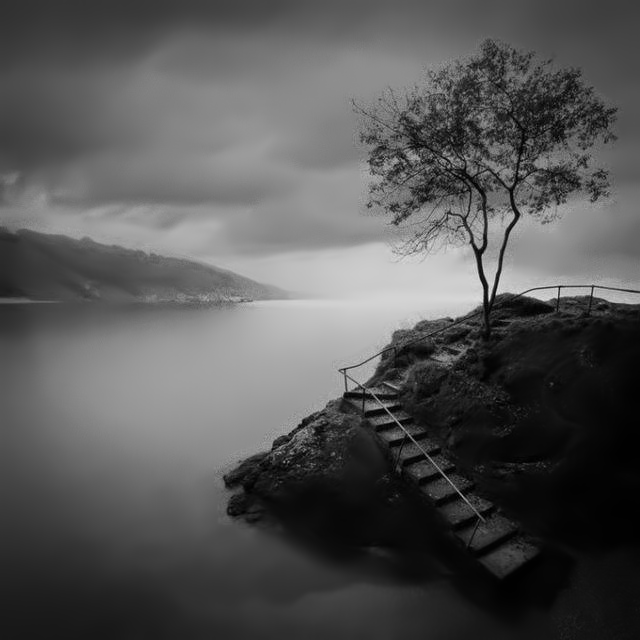
\includegraphics[width=1\linewidth]{images/NLM_op_5_21_21.png} \\ а) fastNlMeansDenoising} 
\end{minipage}
\hfill
\begin{minipage}[h]{0.47\linewidth}
\center{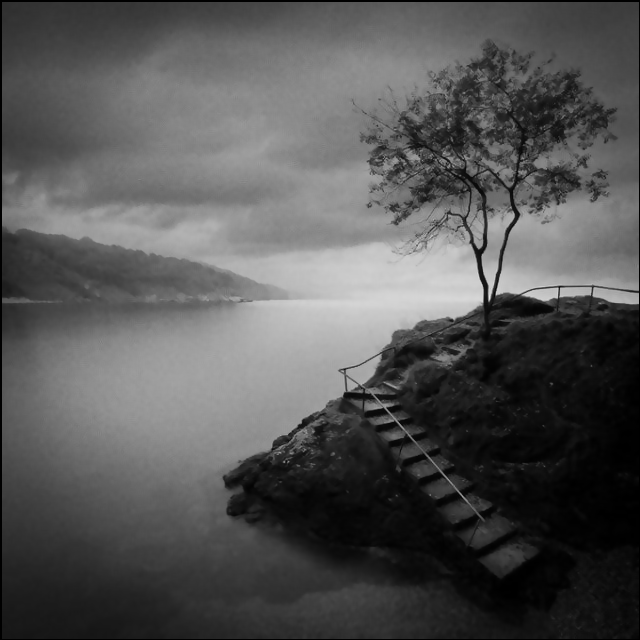
\includegraphics[width=1\linewidth]{images/NLM_5_21.png} \\ б) NLMeansFilterOwn}
\end{minipage}
\caption{Изображение после применения фильтра NLMeans (d = 5, sigma = 21)}
\label{ris:image1}
\end{figure}

Видно, что фильтры хорошо удаляют шум с изображения и даже при больших значениях параметров, детали не теряются.


\section{Вывод}

В работе были рассмотрены следующие алгоритмы сглаживания изображений:
\begin{itemize}
\item Gaussian Blur
\item Bilateral Filter
\item Non – local means.
\end{itemize}

Фильтр Гаусса:  обычно используется в цифровом виде для обработки изображений с целью снижения уровня шума. Однако при ресемплинге он дает сильное размытие изображения. Фильтр Гаусса являеться низкочастотным фильтром. Идеально подходит для бинарных изображений.

Билатеральная фильтрация: довольно медленная, существуют техники ускорения фильтрации. К сожалению, эти техники используют больше памяти, чем обычная фильтрация и поэтому не могут быть напрямую применены для фильтрации цветных изображений.

Non – local means: способ имеет ряд недостатков. В частности, способ требует значительных вычислительных ресурсов. При обработке области с текстурой фильтр привносит некоторое размытие изображения, в то время как для плоских областей он работает хорошо. Поэтому для областей с текстурой необходима некоторая адаптация фильтра. Также требуется некоторая модификация способа для ускорения алгоритма.

Также для подавления шума используют: медианный фильтр, усреднение (box filter) и прочее.


\clearpage
\section{Листинг}
\lstinputlisting{listings/main.cpp}

\end{document}